\chapter{Lunar-Lander-Domäne}\label{sec:LunaLander}
Wir wollen nun untersuchen, wie sich ein Agent mit unserer Strategie in einer anderen Domäne verhält.

\section{Die Umgebung und die Aufgabe}
Wir nutzen für die folgenden Experimente das Toolkit \textit{OpenAi Gym} \cite{x03_openaiGym}. OpenAi Gym ist eine Kollektion von Environments, die für das Trainieren und Vergleichen von diversen Machine-Learning-Algorithmen gedacht sind. Ein wichtiges Kriterium für die Entwickler ist, die Umgebungen so zugänglich wie möglich zu machen.

Wir verwenden für unsere Versuche das Environment \glqq LunarLander-v2\grqq{}. Der Agent soll hierbei lernen, eine kleine, zweidimensionale Raumkapsel auf einer Landeplattform (markiert mit gelben Fahnen) zu landen. Hierbei ist es wichtig, dass das Raumschiff sachte auf dem Boden aufsetzt, ohne dass seine Landefüße beschädigt werden. Eine visuelle Repräsentation des Environments ist in Abbildung \ref{img:lunarLanderExample} dargestellt.

\begin{figure}[h!]
    \centering
    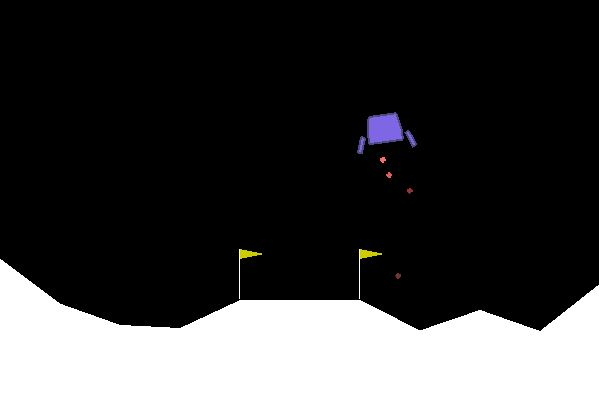
\includegraphics[width=0.7\textwidth]{lunar_lander/lunar_lander_example_image.JPG}
    \caption{OpenAi Gym's \glqq LunarLander-v2\grqq{}} \label{img:lunarLanderExample}
\end{figure}

Zu Beginn jeder Episode spawnt der Lander am oberen Bildschirmrand mit einem zufälligen Winkel und einer leicht variierenden Position. Sein Zustand wird mit sieben Attribute beschrieben: Die horizontale und vertikale Koordinate, die horizontale und vertikale Geschwindigkeit, der Winkel und die Winkelgeschwindikeit der Kapsel und ob die einzelnen Landefüße (2 Stück) den Boden berühren. Die Belohnung hängt von mehreren Komponenten ab: Ob sich der Lander der Landezone nähert oder sich davon entfernt, ob er zum Stillstand kommt oder crasht, ob seine Füße den Boden berühren und natürlich ob er sich in der Landezone befindet. Außerdem erhält er eine kleine Strafe jedes Mal, wenn er das Haupttriebwerk benutzt. Dies ist neben nichts tun, linkes Triebwerk benutzen und rechtes Triebwerk benutzen eine der vier möglichen Aktionen.

Der in diesem Kapitel verwendete Lernalgorithmus ist bis auf kleine Anpassungen mit dem aus Kapitel \ref{sec:deepQImplementation} identisch. Der Hauptunterschied ist, dass dieses Mal ReLu als Activation-Function der Hidden-Layers verwendet wird.

\section{Experimente}
\paragraph{Klassisches $ \epsilon $-greedy}
Wir beginnen wieder mit dem klassischen $ \epsilon $-greedy Ansatz. Nach einigen Vorabtests wählen wir die Hyperparameter wie folgt:
\begin{minted}{python}
params = DeepQParameters(
            num_episodes=2500,
            max_steps_per_episode=0,
            replay_buffer_size=20000,
            batch_size=32,
            learning_rate=0.001,
            discount_rate=0.99,
            target_update=10,
            start_exploration_rate=1,
            max_exploration_rate=1,
            min_exploration_rate=0,
            exploration_decay_rate=0.005,
            # ... Rest wird erst während des Trainings belegt
        )
\end{minted}
Hierbei fällt auf, dass die \mintinline{python}{max_steps_per_episode} auf \mintinline{python}{0} gesetzt sind. Dies liegt daran, dass die maximale Schrittanzahl in der Umgebung intern auf 1000 festgelegt ist. Eine Episode endet außerdem, sobald der Lander das Bild verlässt, crasht oder zum Stillstand kommt. Aufgrund der sehr langen Trainingszeit beschränken wir die Anzahl der Iterationen pro Experiment auf 10.

\begin{figure}[h!]
    \centering
    \begin{subfigure}[b]{0.7\textwidth}
        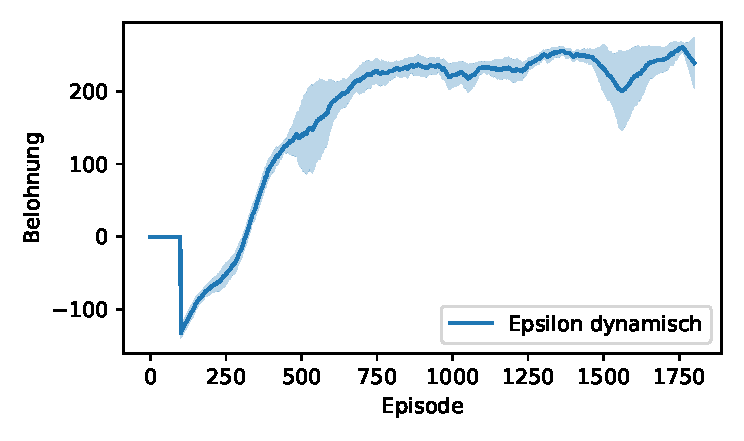
\includegraphics[width=\textwidth]{lunar_lander/figure_classic_epsilon.pdf}
        \caption{Graph so wie in \ref{img:graphQEpsComp}.}
        \label{img:lunarClassicEps01Graph}
    \end{subfigure}
    \begin{subfigure}[b]{0.5\textwidth}
        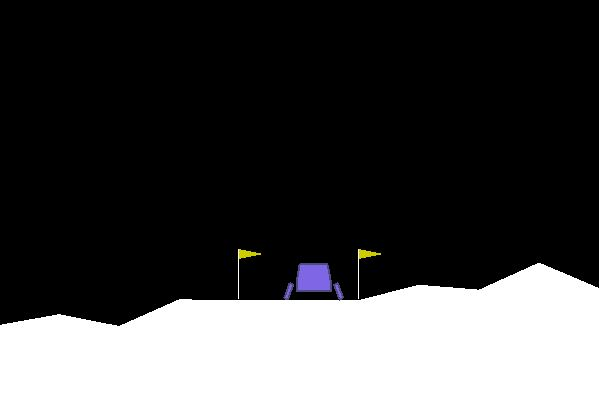
\includegraphics[width=\textwidth]{lunar_lander/lunar_lander_decaying_epsilon.JPG}
        \caption{Gelandeter Lander unter Verwendung des trainierten DQNs}
        \label{img:lunarClassicEps01Env}
    \end{subfigure}
    \caption{Trainingsergebnisse mit dynamischem $ \epsilon $ nach 10 Wiederholungen.} \label{img:lunarClassicEps01}
\end{figure}

Abbildung \ref{img:lunarClassicEps01} zeigt die Ergebnisse des ersten Experiments. Der Graph \ref{img:lunarClassicEps01Graph} zeigt wieder den durchschnittlichen moving average mitsamt seiner Standardabweichung. Die Belohnung steigt bis Episode 750 stetig an und pendelt sich dann bei einem Wert von ungefähr 230 ein. Gegen Ende circa bei Episode 1500 bricht der Plot nochmal leicht ein, steigt aber danach wieder an. Die Standardabweichung ist an den meisten Stellen gering. Die Lernkurve verläuft also weitestgehend wie gewünscht. Auch das Resultat ist sehr positiv, da der Agent unter Anwendung der trainierten DQNs den Lander in den meisten Fällen schnell aber sanft in der Zielzone landet.

\paragraph{Training ohne Erkundungsstrategie}
Wir wollen nun wieder die unterschiedlichen Ansätze miteinander vergleichen. Um zunächst zu sehen, wie das Training ohne eine Erkundungsstrategie verläuft, setzen wir unser $ \epsilon $ wieder konstant auf 0.

\begin{figure}[h!]
    \centering
    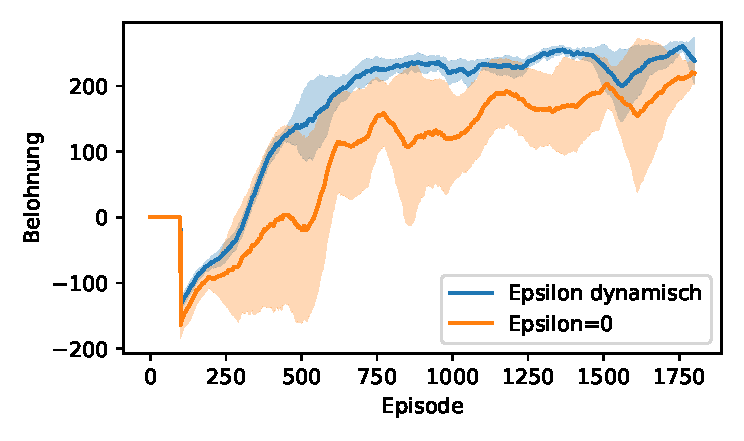
\includegraphics[width=0.7\textwidth]{lunar_lander/figure_classic_epsilon_vs_no_exploration.pdf}
    \caption{Graph so wie in \ref{img:graphQEpsComp}. Vergleich der Trainingsverläufe mit dynamischem $ \epsilon $ (blau) und statischem $ \epsilon = 0.0 $ bzw. keiner Erkundungsstrategie (gelb).} \label{img:lunarClassicEps01VsNoExploration}
\end{figure}

Wie erwartet zeigt der Graph in Abbildung \ref{img:lunarClassicEps01VsNoExploration}, dass das Training ohne Erkundungsstrategie schlechtere Ergebnisse liefert. Die durchschnittliche Belohnung steigt nicht so schnell an wie im letzten Experiment und die Standardabweichung ist größer. Der Lernfortschritt ist also langsamer und inkonsistenter als zuvor, was auch hier klar für die Verwendung der $ \epsilon $-greedy Strategie spricht.

\paragraph{Training mit modifiziertem Reward}
Zuletzt bilden wir die Erkundungsstrategie wieder ausschließlich im Reward ab. Wir nutzen hierfür die Ergebnisse aus Kapitel \ref{sec:deepQRewardModification} und multiplizieren die Belohnung, die die Umgebung zurückgibt, mit \mintinline{python}{(1 - exploration_rate)}:
\begin{minted}{python}
modified_reward = (1 - exploration_rate) * reward
\end{minted}
Damit der Agent zu Beginn überhaupt eine Belohnung bekommt starten wir mit einer \mintinline{python}{exploration_rate} von 0.5, die \mintinline{python}{start_exploration_rate} und \mintinline{python}{max_exploration_rate} werden also auf 0.5 gesetzt. Der Agent agiert für dieses Experiment wieder ausschließlich greedy.

\begin{figure}[h!]
    \centering
    \begin{subfigure}[b]{0.49\textwidth}
        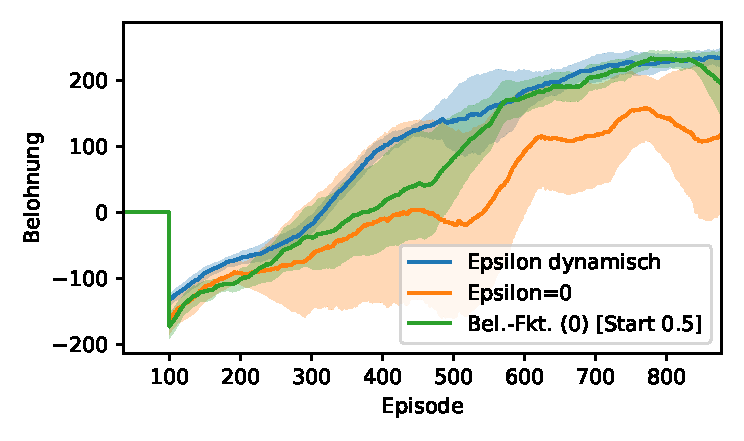
\includegraphics[width=\textwidth]{lunar_lander/figure_comparison_all_01_big_1.pdf}
        \caption{Ausschnitt des linken Startbereichs}
        \label{img:lunarComparisonAll01Big1}
    \end{subfigure}
    \begin{subfigure}[b]{0.49\textwidth}
        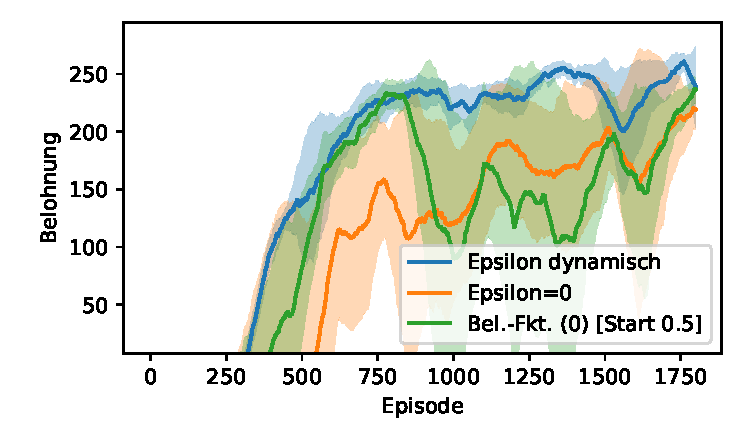
\includegraphics[width=\textwidth]{lunar_lander/figure_comparison_all_01_big_2.pdf}
        \caption{Ausschnitt des oberen Bereichs}
        \label{img:lunarComparisonAll01Big2}
    \end{subfigure}
    \begin{subfigure}[b]{0.7\textwidth}
        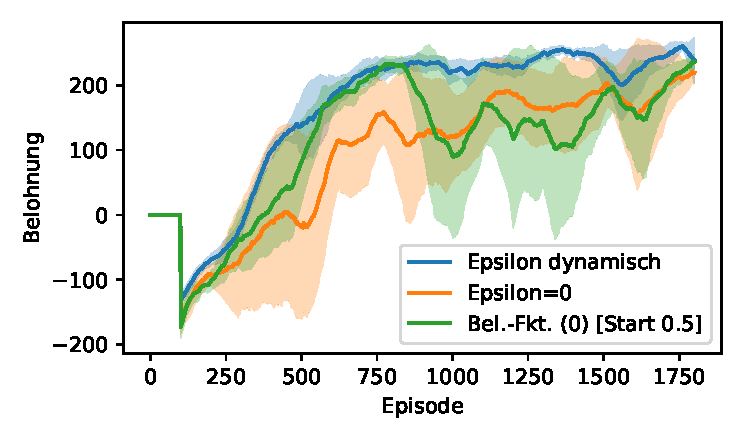
\includegraphics[width=\textwidth]{lunar_lander/figure_comparison_all_01.pdf}
        \caption{Kompletter Plot}
        \label{img:lunarComparisonAll01}
    \end{subfigure}
    \caption{Graphen so wie in \ref{img:graphQEpsComp}. Vergleich der Trainingsverläufe mit dynamischem $ \epsilon $ (blau), statischem $ \epsilon = 0.0 $ (gelb) und modifiziertem Reward mit Faktor 0 mit \mintinline{python}{start_exploration_rate=0.5} (grün) nach jeweils 20 Wiederholungen.}
    \label{img:lunarComparisonAll01All}
\end{figure}

Wir vergleichen den Verlauf des Trainings mit denen der vorangegangenen Experimente. Für den Vergleich haben wir in diesem Versuch selbstverständlich wieder den echten Reward der Umgebung genommen. Betrachten wir zunächst die ersten 800 Episoden, dargestellt in Abbildung \ref{img:lunarComparisonAll01Big1}. Die Belohnung steigt etwas schneller an als bei $ \epsilon = 0 $ und die Standardabweichung ist geringer. In Episode 800 liegt der Belohnungswert etwa auf gleicher Höhe mit dem der klassischen $ \epsilon $-greedy Strategie. Es sieht so aus, als würde sich unsere Strategie hier besser schlagen als ein Agent ohne Erkundungsstrategie. Betrachten wir nun allerdings den Verlauf nach Episode 800, gut zu erkennen in Abbildung \ref{img:lunarComparisonAll01Big2}, so fällt auf, dass der moving average sogar unter den Wert vom Experiment mit $ \epsilon = 0 $ fällt. Die Standardabweichung bricht hier ebenfalls sehr stark aus. Beides bessert sich erst gegen Ende des Trainings wieder. Diese Tatsache lässt unsere Strategie hier nicht ganz so gut aussehen. Es lässt sich deswegen keine absolut klare Aussage über einen definitiven Vorteil unserer Strategie gegenüber dem Nichtverwenden einer Erkundungsstrategie treffen.

Betrachten wir noch die Boxplots aus Abbildung \ref{img:lunarComparisonAllBox01Both} für die Experimente nach jeweils 100 Durchläufen mit den jeweiligen DQNs.
\begin{figure}[h!]
    \centering
    \begin{subfigure}[b]{0.7\textwidth}
        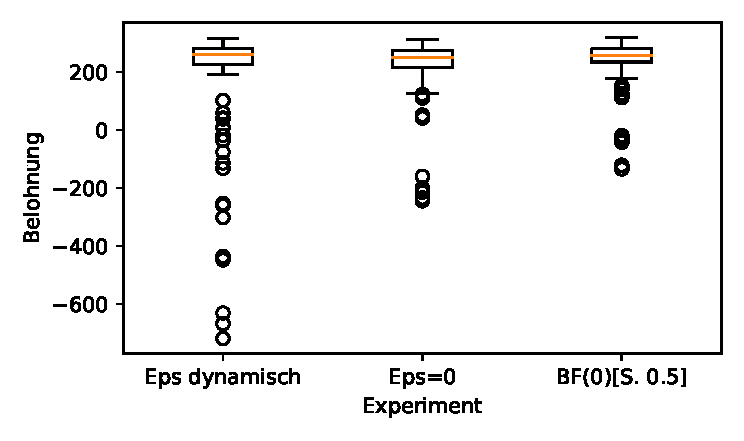
\includegraphics[width=\textwidth]{lunar_lander/figure_comparison_all_01_box.pdf}
        \caption{Kompletter Plot}
        \label{img:lunarComparisonAllBox01}
    \end{subfigure}
    \begin{subfigure}[b]{0.7\textwidth}
        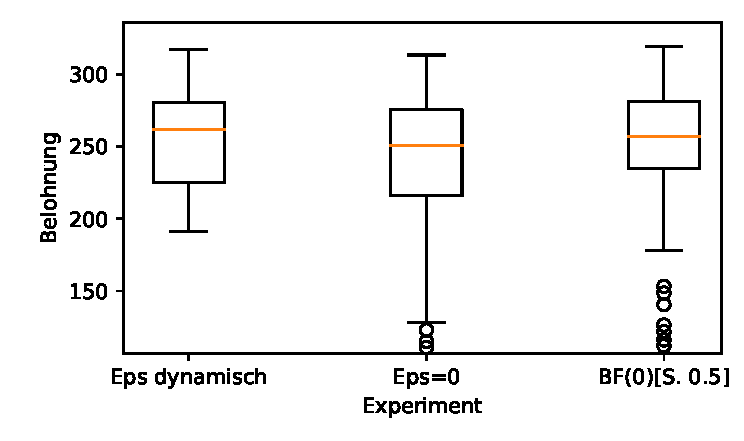
\includegraphics[width=\textwidth]{lunar_lander/figure_comparison_all_01_box_big.pdf}
        \caption{Ausschnitt ohne die unteren Ausreißer}
        \label{img:lunarComparisonAllBox01Big}
    \end{subfigure}
    \caption{Boxplots so wie in \ref{img:graphBoxEpsComparisonBoth}. Experimente von links nach rechts: $ \epsilon $ dynamisch, $ \epsilon = 0.0 $, modifizierter Reward mit Faktor 5, modifizierter Reward mit Faktor 0 mit \mintinline{python}{start_exploration_rate=0.5}.}
    \label{img:lunarComparisonAllBox01Both}
\end{figure}
Wie erwartet ist der Median beim klassischen $ \epsilon $-greedy Ansatz am größten, wenn auch nicht um viel. Vergleichen wir die letzten beiden Versuche miteinander, so lässt sich erkennen, dass alle Quantile unseres Experiments über denen des Versuchs ohne Erkundungsstrategie liegen. Unser Ansatz scheint etwas bessere Ergebnisse zu liefern als ein Training ohne Erkundungsstrategie und der Boxplot kann dem der $ \epsilon $-greedy-Strategie fast das Wasser reichen. Allerdings lässt sich anhand dieser Daten schwer eine endgültige Aussage hierüber treffen. Erforderlich wären eine größere Episodenanzahl, wesentlich mehr Iteration pro Experiment und weitere Durchläufe zum Anpassen der Hyperparameter. Hierfür fehlen uns für diese Domäne im Zuge dieser Arbeit die erforderlichen Rechenressourcen.

% Der Graph \ref{img:graphClassicEps01} zeigt wieder den durchschnittlichen moving average mitsamt seiner Standardabweichung. Der Agent scheint bis Episode 1000 einen sehr ordentlichen Lernfortschritt zu machen. Die Lernkurve beginnt hier steil und flacht dann langsam ab, so wie es wünschenswert ist. Nach Epsiode 1000 fällt die Kurve allerdings nochmals stark ab und die Standardabweichung bricht stark aus. Kurz darauf steigt der Wert wieder und erreicht ein neues Maximum, bevor er wieder leicht abfällt. Der Agent landet den Lander bei der Anwendung des DQNs relativ ruppig und lässt nach der Landung meist die seitlichen Triebwerke laufen.

% Da dieses Verhalten noch nicht optimal ist und der Graph gegen Ende ziemlich kurvig wird, führen wir das Experiment nochmals mit 2500 Episoden durch. Da eine Iteration dieses Experiments deutlich länger dauert als beim Navigations-Problem, setzen wir die Wiederholungen pro Experiment auf 10 herab, um die Versuche in absehbarer Zeit durchführen zu können.

% \begin{figure}[h!]
%     \centering
%     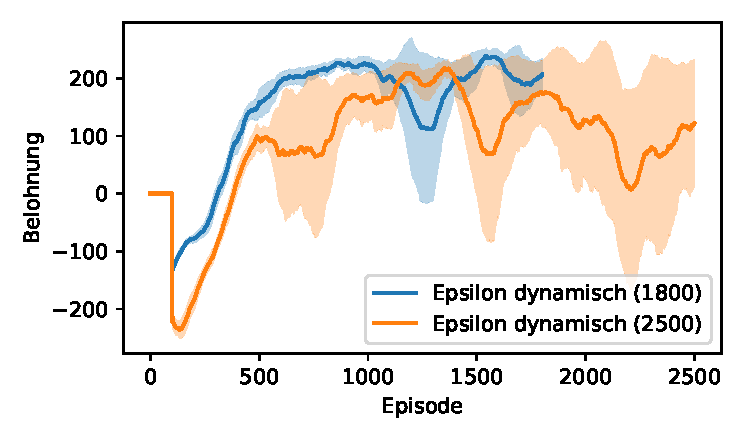
\includegraphics[width=0.7\textwidth]{lunar_lander/figure_classic_epsilon_02.pdf}
%     \caption{TODO} \label{img:graphClassicEps02}
% \end{figure}

% In Graph \ref{img:graphClassicEps02} ist zu sehen, dass das neue Experiment (orange) trotz (bis auf die Episodenanzahl) identischer Parameter etwas anders verläuft als das letzte. Der Belohnungsdurchschnitt erreicht etwa dort seinen Höhepunkt, wo der vorangegangene Versuch nochmals eingebrochen ist und umgekehrt. Wir vermuten, dass dies an der sensiblen Umgebung liegen kann. Eine kleine Aktion hat hier eine relativ große Auswirkung. So kann beispielsweise das Zünden eines der Steuertriebwerke im falschen Moment zum Kippen des Landers und somit zum Crash führen.

% Nichtsdestotrotz zeigen einige Stichproben mit den gelernten DQNs, dass der Agent durchaus meistens nach dem Training dazu in der Lage ist, das Raumschiff sehr sanft und zielgenau zu landen. Dies wird wahrscheinlich dadurch ermöglicht, dass wir auch hier am Ende das Netz ausgeben, welches während des Trainings den höchsten moving average produziert hat.

% TODO Boxplots












% \section{Experimente}
% \paragraph{Klassisches $ \epsilon $-greedy}
% Wir beginnen wieder mit dem klassischen $ \epsilon $-greedy Ansatz. Außerdem ist die Episodenanzahl aus dem gleichen Grund verhältnismäßig gering gewählt. Nach einigen Vorabtests haben sich die folgenden Hyperparameter herauskristallisiert:
% \begin{minted}{python}
% params = DeepQParameters(
%             num_episodes=1800,
%             max_steps_per_episode=0,
%             replay_buffer_size=20000,
%             batch_size=32,
%             learning_rate=0.001,
%             discount_rate=0.99,
%             target_update=10,
%             start_exploration_rate=1,
%             max_exploration_rate=1,
%             min_exploration_rate=0,
%             exploration_decay_rate=0.005,
%             # ... Rest wird erst während des Trainings belegt
%         )
% \end{minted}
% Hierbei fällt auf, dass die \mintinline{python}{max_steps_per_episode} auf \mintinline{python}{0} gesetzt sind. Dies liegt daran, dass eine Episode endet, sobald der Lander das Bild verlässt, crasht oder zum Stillstand kommt.

% \begin{figure}[h!]
%     \centering
%     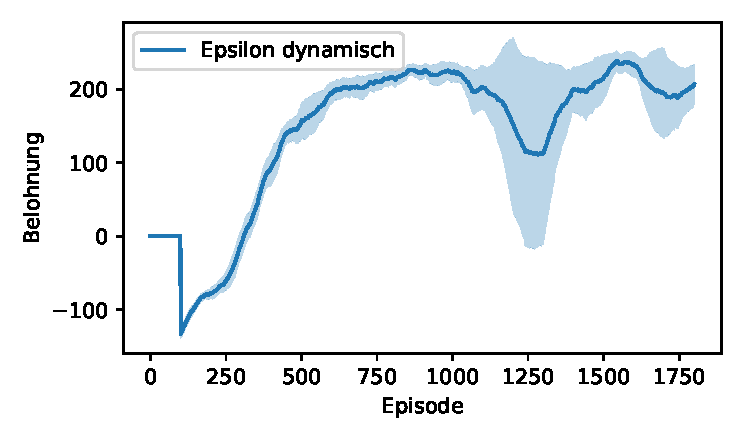
\includegraphics[width=0.7\textwidth]{lunar_lander/figure_classic_epsilon_01.pdf}
%     \caption{TODO} \label{img:graphClassicEps01}
% \end{figure}

% Der Graph \ref{img:graphClassicEps01} zeigt wieder den durchschnittlichen moving average mitsamt seiner Standardabweichung. Der Agent scheint bis Episode 1000 einen sehr ordentlichen Lernfortschritt zu machen. Die Lernkurve beginnt hier steil und flacht dann langsam ab, so wie es wünschenswert ist. Nach Epsiode 1000 fällt die Kurve allerdings nochmals stark ab und die Standardabweichung bricht stark aus. Kurz darauf steigt der Wert wieder und erreicht ein neues Maximum, bevor er wieder leicht abfällt. Der Agent landet den Lander bei der Anwendung des DQNs relativ ruppig und lässt nach der Landung meist die seitlichen Triebwerke laufen.

% Da dieses Verhalten noch nicht optimal ist und der Graph gegen Ende ziemlich kurvig wird, führen wir das Experiment nochmals mit 2500 Episoden durch. Da eine Iteration dieses Experiments deutlich länger dauert als beim Navigations-Problem, setzen wir die Wiederholungen pro Experiment auf 10 herab, um die Versuche in absehbarer Zeit durchführen zu können.

% \begin{figure}[h!]
%     \centering
%     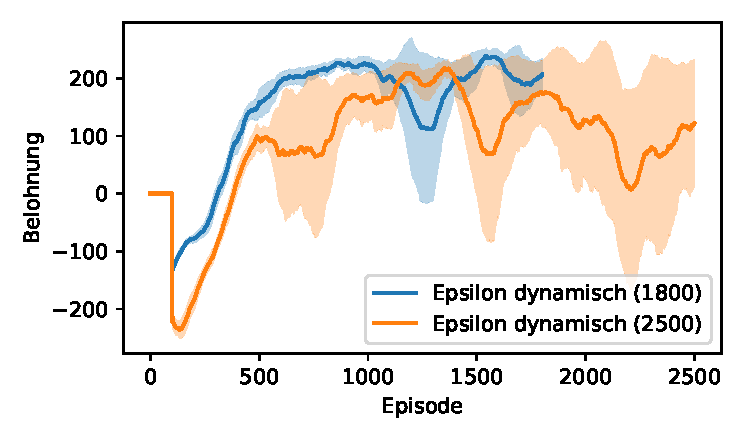
\includegraphics[width=0.7\textwidth]{lunar_lander/figure_classic_epsilon_02.pdf}
%     \caption{TODO} \label{img:graphClassicEps02}
% \end{figure}

% In Graph \ref{img:graphClassicEps02} ist zu sehen, dass das neue Experiment (orange) trotz (bis auf die Episodenanzahl) identischer Parameter etwas anders verläuft als das letzte. Der Belohnungsdurchschnitt erreicht etwa dort seinen Höhepunkt, wo der vorangegangene Versuch nochmals eingebrochen ist und umgekehrt. Wir vermuten, dass dies an der sensiblen Umgebung liegen kann. Eine kleine Aktion hat hier eine relativ große Auswirkung. So kann beispielsweise das Zünden eines der Steuertriebwerke im falschen Moment zum Kippen des Landers und somit zum Crash führen.

% Nichtsdestotrotz zeigen einige Stichproben mit den gelernten DQNs, dass der Agent durchaus meistens nach dem Training dazu in der Lage ist, das Raumschiff sehr sanft und zielgenau zu landen. Dies wird wahrscheinlich dadurch ermöglicht, dass wir auch hier am Ende das Netz ausgeben, welches während des Trainings den höchsten moving average produziert hat.

% TODO Boxplots